\setAuthor{Mihkel Pajusalu}
\setRound{piirkonnavoor}
\setYear{2011}
\setNumber{G 2}
\setDifficulty{1}
\setTopic{Taevamehaanika}

\prob{Satelliit}
Satelliit tiirleb ringikujulisel orbiidil (raadiusega $r=\SI{7000}{\kilo\metre}$) ümber maakera, kusjuures satelliidi orbiit on samas tasapinnas Maa orbiidiga ümber Päikese. Kui suure osa ajast keskmiselt veedab satelliit Maa varjus? Maa läbimõõt on $R=\SI{6378}{\kilo\metre}$. Päikeselt tulevad kiired võib lugeda paralleelseteks ja Maa liikumise ühe satelliidi orbiiditaalperioodi jooksul tühiseks.

\hint
Ringikujulisel orbiidil on satelliidi kiirus kogu orbitaalperioodi jooksul konstantne ja seetõttu on varjus veedetud osa ajast võrdne orbiidi varjus oleva osa pikkuse ja kogu orbiidi pikkuse suhtega.

\solu
\begin{center}
	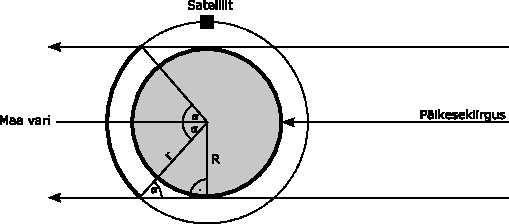
\includegraphics[width=0.9\linewidth]{2011-v2g-02-lah}
\end{center}
Ringikujulisel orbiidil on satelliidi kiirus kogu orbitaalperioodi jooksul konstantne ja seetõttu on varjus veedetud osa ajast võrdne orbiidi varjus oleva osa pikkuse ja kogu orbiidi pikkuse suhtega, mis on ülal toodud jooniselt leitav kui 
\[
k=\frac{2 \alpha r}{2 \pi r}=\frac{\arcsin \left(\frac{R}{r}\right)}{\pi}=\SI{36,5}{\%}
\]
\probend